\documentclass[xcolor={table}]{beamer}
%\usetheme{Lapesd}
\usepackage{./sty/beamerthemeLapesd}

\usepackage{morewrites}

\usepackage[brazilian]{babel}	% coloca as coisas em portugues no sumário.
\usepackage[utf8]{inputenc}
\usepackage[T1]{fontenc}
\usepackage[scaled]{helvet}
\usepackage{amsthm}
\usepackage{ragged2e}
% \usepackage{subfig}
\usepackage[table]{xcolor}
\usepackage{ctable}
\usepackage{multicol}
\usepackage{multirow}
\usepackage{fancyvrb}
\usepackage{subcaption}
\usepackage{listings}
\usepackage{color}
\usepackage[font={scriptsize,it}]{caption}
\renewcommand{\lstlistingname}{Code}
\definecolor{lightgray}{rgb}{0.97,0.97,0.97}
\definecolor{lightred}{rgb}{1,0.7,0.7}

\lstdefinelanguage{cc}{
    language     = C++,
    morekeywords = {Array2D, __parallel__, Mask2D, Stencil2D}
}

\lstdefinestyle{highlight}{
    numbers=none,
    stepnumber=1,
    numbersep=-8pt,
    numberstyle=\small\color{black},
    basicstyle=\scriptsize\ttfamily\color{black},
    keywordstyle=\color{blue},
    commentstyle=\color{black},
    stringstyle=\color{black},
    numberstyle=\footnotesize\ttfamily\color{black},
    escapeinside={(*}{*)},
    tabsize=2,
    language=cc, %morecomment=[l][{\color[rgb]{0.1, 0.2, 0.8}}]{},
    %aboveskip=0.1in, % space before the caption
    %belowskip=0.1in, % space after listing
    captionpos=b,
    showstringspaces=false,
    %belowcaptionskip=1\baselineskip,
    %breaklines=true,
    %moredelim=[l][\color{blue}]{\#pragma},
    % backgroundcolor=\color{white}
}

\lstdefinestyle{base}{
    numbers=none,
    stepnumber=1,
    numbersep=-8pt,
    morekeywords={Array2D, \_\_parallel\_\_, Mask2D, Stencil2D}
    numberstyle=\small\color{black!40},
    basicstyle=\scriptsize\ttfamily\color{black!40},
    keywordstyle=\color{blue!40},
    commentstyle=\color{black!40},
    stringstyle=\color{black!40},
    numberstyle=\footnotesize\ttfamily\color{black!40},
    escapeinside={(*}{*)},
%     frame=none, %single
    tabsize=2,
    language=cc, %morecomment=[l][{\color[rgb]{0.1, 0.2, 0.8}}]{},
    %aboveskip=0.1in, % space before the caption
    %belowskip=0.1in, % space after listing
    captionpos=b,
    showstringspaces=false,
    %belowcaptionskip=1\baselineskip,
    %breaklines=true,
    %moredelim=[l][\color{blue}]{\#pragma},
    % backgroundcolor=\color{white!40}
    moredelim=**[is][\only<+>{\color{black}\lstset{style=highlight}}]{@}{@},
}

% \lstdefinestyle{highlight}{
    % keywordstyle=\color{red},
    % commentstyle=\color{green},
% }
% \lstdefinestyle{base}{
    % language={C++},
    % basicstyle=\color{black!40},
    % keywordstyle=\color{red!40},
    % commentstyle=\color{green!40},
    % moredelim=**[is][\only<+>{\color{black}\lstset{style=highlight}}]{@}{@},
% }

\newcommand{\Fw}{\textit{Framework}\xspace}
\newcommand{\fw}{\textit{framework}\xspace}
\newcommand{\Fws}{\textit{Frameworks}\xspace}
\newcommand{\fws}{\textit{frameworks}\xspace}

\newcommand{\pskel}{PSkel\xspace}
\newcommand{\mppa}{MPPA-256\xspace}

\graphicspath{{./figs/}}
\DeclareGraphicsExtensions{.pdf,.jpg,.png,.gif}

\def\signed #1{{\leavevmode\unskip\nobreak\hfil\penalty50\hskip2em
        \hbox{}\nobreak\hfil(#1)
        \parfillskip=0pt \finalhyphendemerits=0 \endgraf}}

\renewcommand{\footnotesize}{\tiny}

\newcommand{\mymacro}[1]{#1}

\addtobeamertemplate{block begin}{}{\justifying}

\captionsetup{labelformat=simple}
\captionsetup[table]{belowskip=0pt}

\title[Otimização de aplicações do CAP Bench para o MPPA-256]{
   \textbf{Otimização de aplicações do CAP Bench para o processador MPPA-256}}
\author[Grunheidt, D.]{\textbf{David Grunheidt Vilela Ordine}, Emmanuel Podestá Jr., \\Pedro Henrique Penna, Márcio Castro}
\date{11 de abril de 2019}
\institute{Departamento de Informática e Estatística (INE)\\ Universidade Federal de Santa Catarina (UFSC)\\ 
\url{david.ordine@grad.ufsc.br} \\ \url{emmanuel.podesta@posgrad.ufsc.br} \\ \url{pedro.penna@univ-grenoble-alpes.fr} \\ \url{marcio.castro@ufsc.br}}

\begin{document}
\begingroup
    \makeatletter
    \setlength{\hoffset}{-0.5\beamer@sidebarwidth}
    \makeatother
    \begin{frame}[plain,t,noframenumbering]
        \titlepage
    \end{frame}
\endgroup

%=============================================================================================

\section{Sumário}
\begin{frame}\frametitle{Sumário}
    \begin{itemize}
        \item Introdução
        \item Fundamentação Teórica
        \item CAP Bench Otimizado
        \item Resultados dos experimentos
        \item Conclusão
    \end{itemize}

    \vfill
\end{frame}

\section{Introdução}

\begin{frame}\frametitle{Contexto}
    \subsection{Contexto}
    \begin{itemize}
        \item{Objetivo de alcançar a computação em \textit{Exaescale}}
        \item{\textit{Trade-off} desproporcional entre alto desempenho e consumo energético viável (barreira de potência)}
        \item{Processadores \textit{manycore} de baixa potência como solução do problema}
        \begin{itemize}
            \item {MPPA-256 \cite{MPPA-2:2013}}
            \item {Adapteva Epiphany \cite{Olofsson2014}}
            \item {SW26010 (\textit{Sunway TaihuLight}) \cite{sunway:2016}}
        \end{itemize}
    \end{itemize}

    \vfill
\end{frame}

\begin{frame}\frametitle{Contexto}
    \begin{itemize}
        \item {Necessário avaliar o desempenho do MPPA-256}
        \begin{itemize}
            \item CAP-Benchmarks
        \end{itemize}
        \item {Versão do benchmark já ultrapassada}
        \begin{itemize}
            \item Baixo nível de abstração
            \item Acesso lento a dados localizados em memorias remotas
        \end{itemize}
        \item {\textbf{Objetivo:}}
        \begin{itemize}
        	\item Criar uma nova versão para o \textit{Benchmark}
            \item Aumentar o nível de abstração
            \item Abstrair o modelo de memoria distribuída
            \item Ganho de desempenho em relação a antiga
        \end{itemize}
    \end{itemize}
    \vfill
    % \textbf{Como podemos simplificar o desenvolvimento?}
\end{frame}

\section{Fundamentação Teórica}
\begin{frame}\frametitle{MPPA-256}
    \subsection{MPPA-256}
    \begin{itemize}
        \item{16 \textit{clusters} de computação (CCs)}
        \begin{itemize}
            \item 16 núcleos em cada CC, atuando a 400 Mhz cada
            \item Memória compartilhada de 2MB
            \item Memória cache associativa 2-way, privadas e de 32 kB
        \end{itemize}
        \item{4 \textit{clusters} de E/S}
        \begin{itemize}
            \item 4 núcleos gerenciadores de recursos em cada
        \end{itemize}
        \begin{figure}
            \centering
            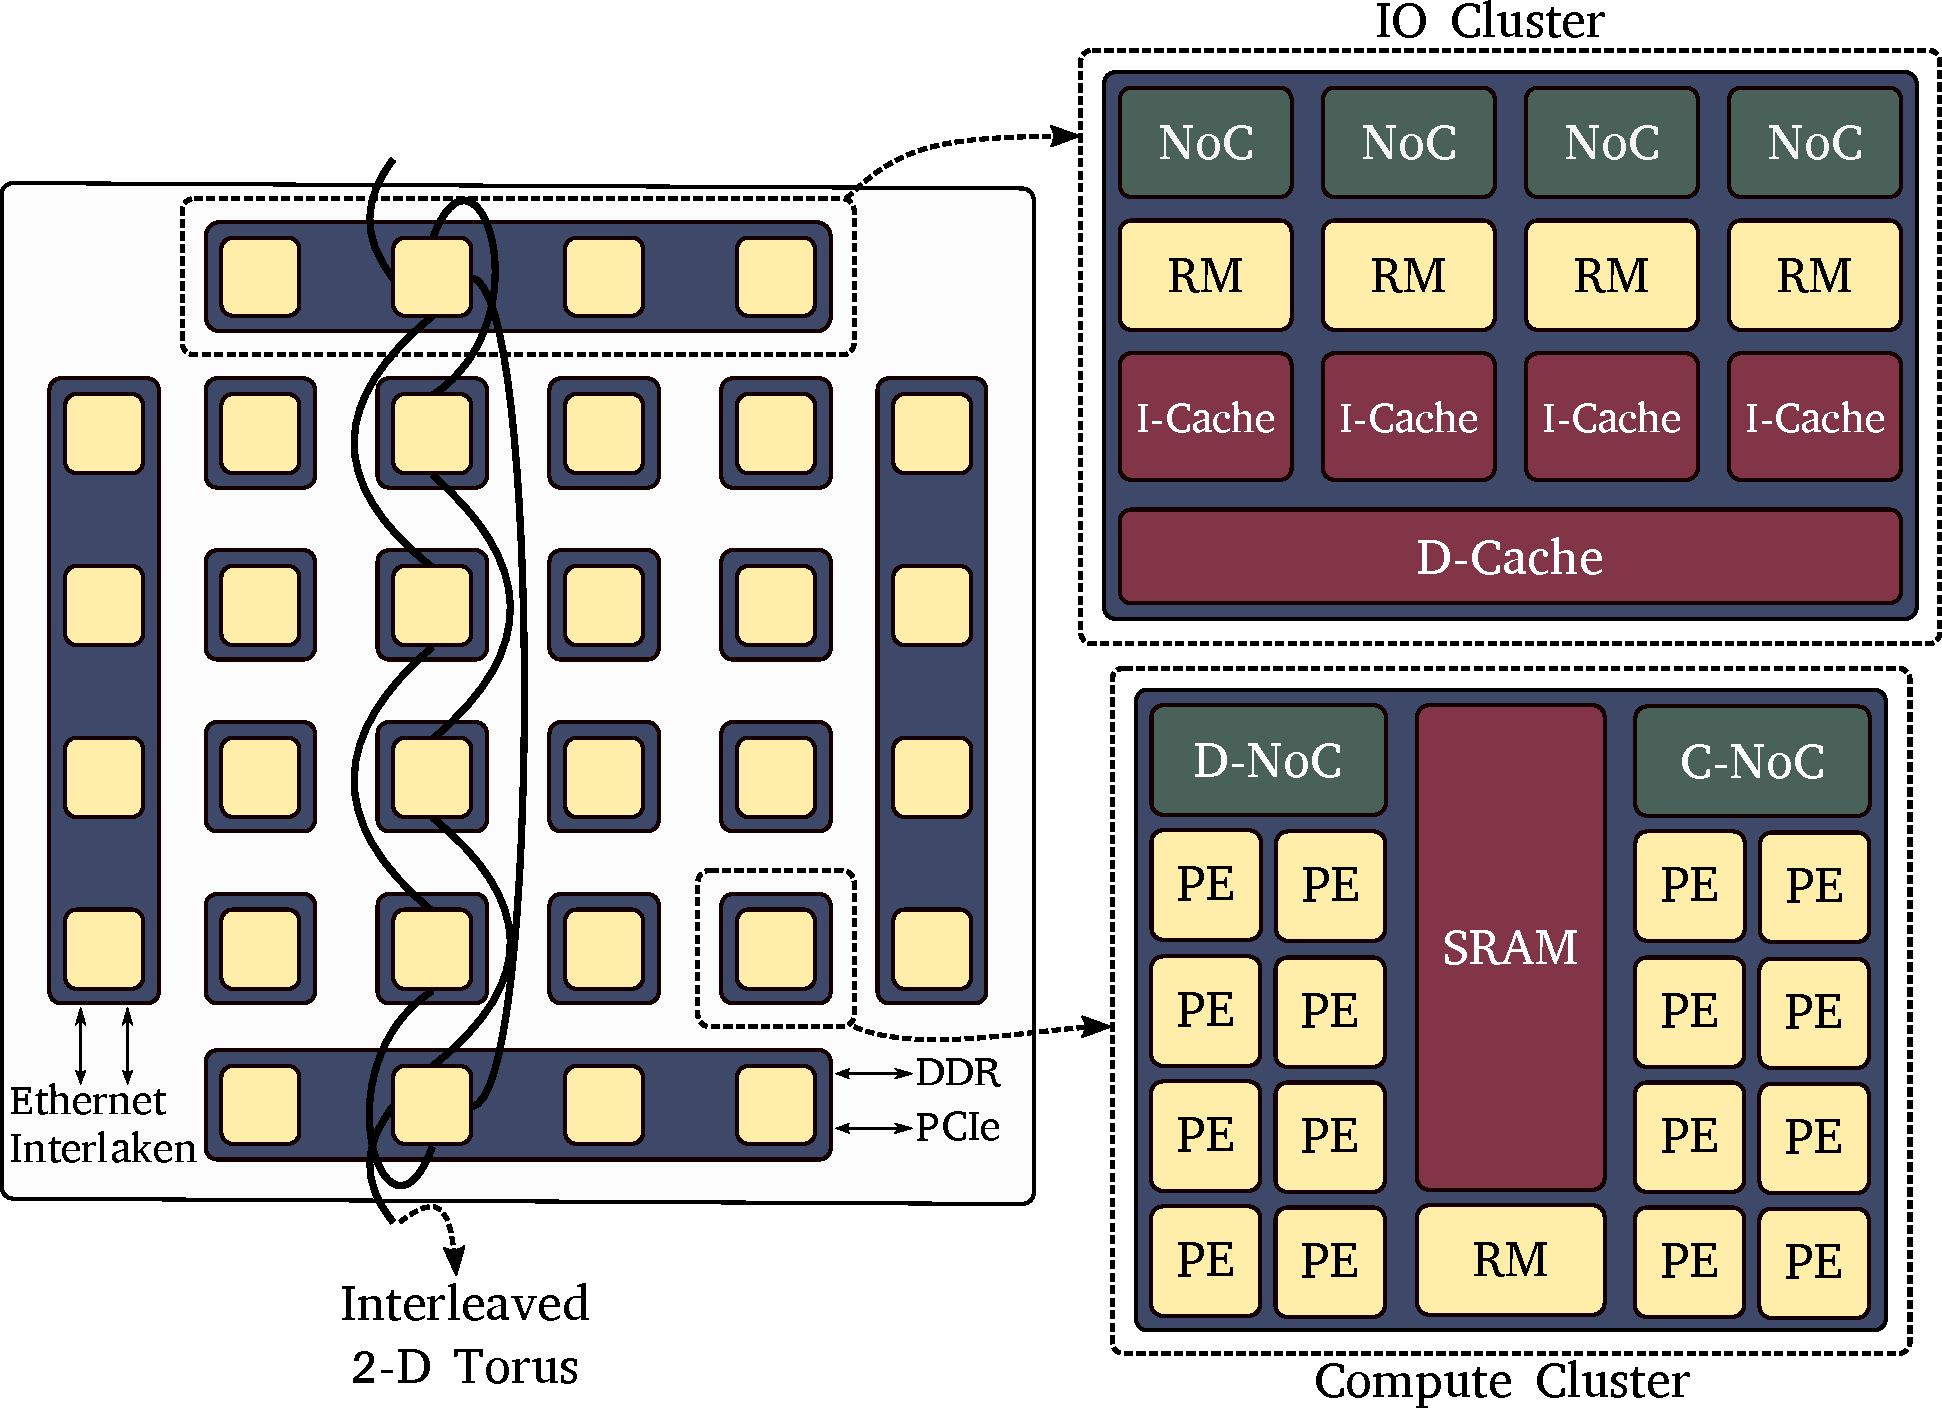
\includegraphics[width=5cm, keepaspectratio]{figs/mppa-overview.pdf}
            \caption{Visão arquitetural do MPPA-256 \cite{Penna2018}}
            \label{fig:rhs+}
        \end{figure}
    \end{itemize}
\end{frame}

\begin{frame}\frametitle{CAP-Benchmarks \cite{Castro-Souza-CCPE:2016}}
    \subsection{CAP-Benchmarks}
    \begin{itemize}
        \item {Conjunto de 7 aplicações desenvolvidas em C}
    	\item {Domínios de problemas variados}
    	\item {Diferentes padrões paralelos}
    	\item {Testar o processador em diversas condições}
    \end{itemize}
\end{frame}

\section{CAP-Bench Otimizado}
\subsection{Async API}
\begin{frame}\frametitle{MPPA ASYNC API \cite{Hascoet2017}}
    \begin{itemize}
        \item {Comunicação assíncrona e unilateral entre \textit{clusters}}
        \item {Segmentos sobre espaços locais de memória}
    	\begin{itemize}
        	\item Abstração do modelo de memoria distribuída
        	\item Clonagem de segmentos
        	\item Operações \textit{put/get} sobre segmentos
    	\end{itemize}
		\begin{figure}
    	\centering
        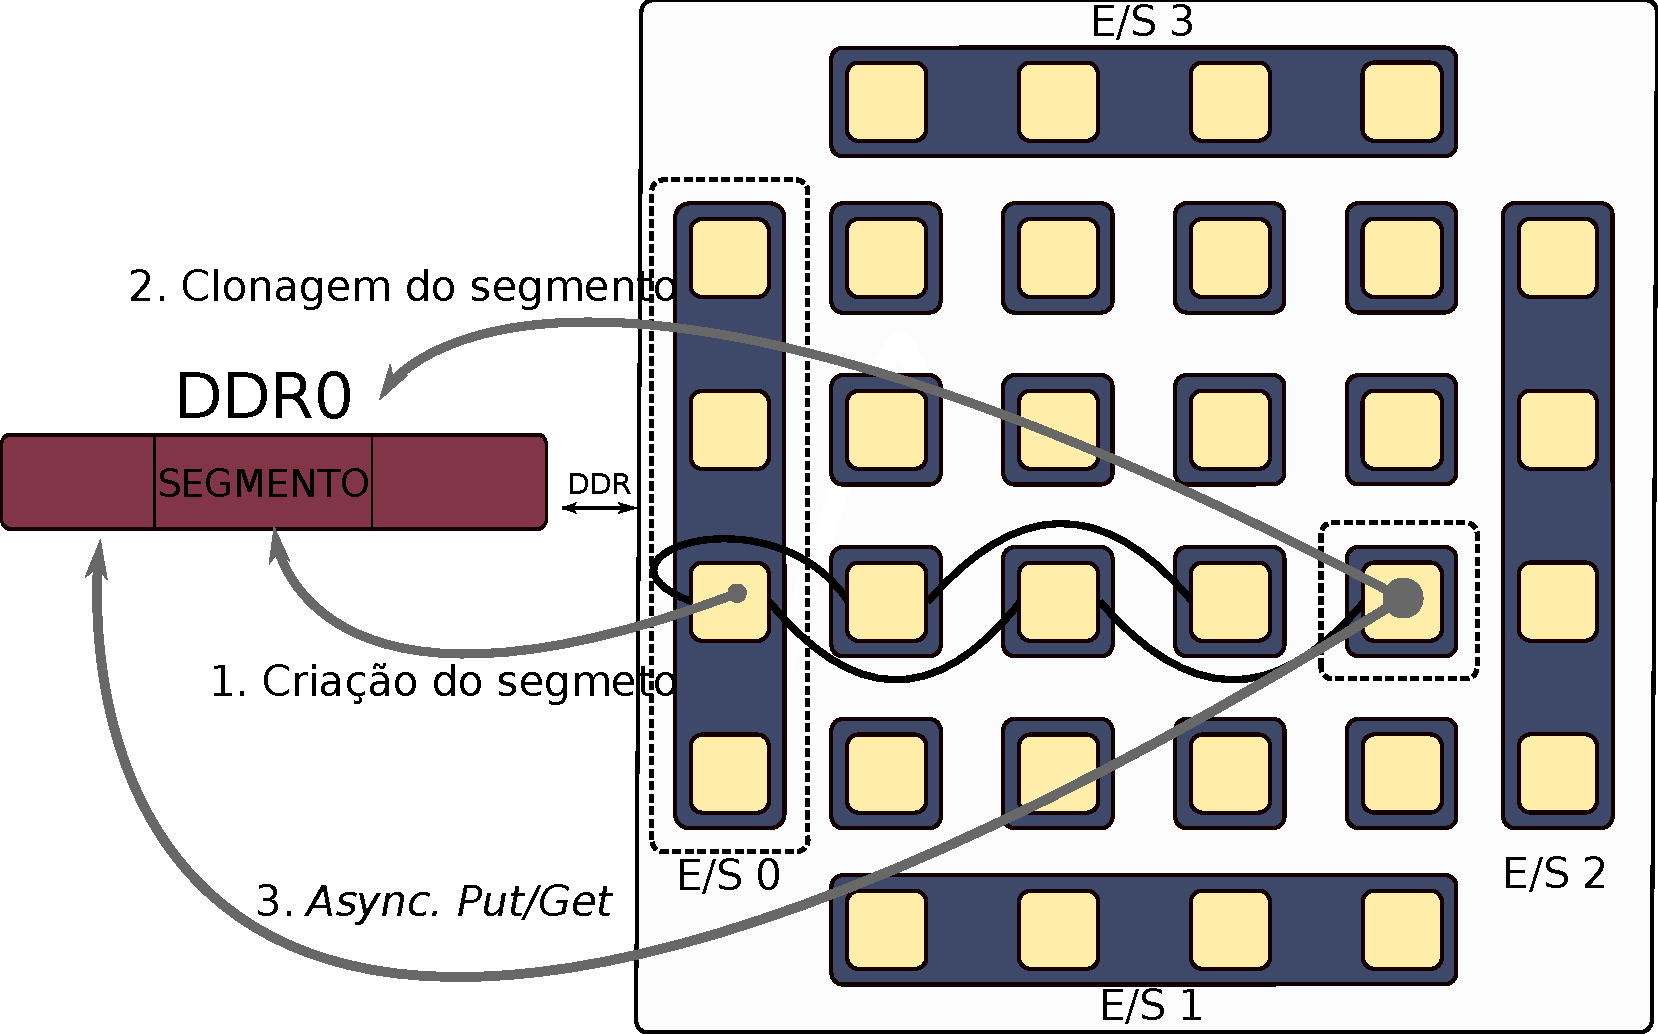
\includegraphics[width=7cm, keepaspectratio]{figs/putget.pdf}\caption{Visão esquemática do funcionamento da biblioteca \textit{async}}\label{fig:putget}
		\end{figure}
    \end{itemize}
\end{frame}

\begin{frame}\frametitle{Friendly Numbers}
    \subsection{Aplicações Portadas}
    \begin{itemize}
    \item Números com a mesma abundância $\mathnormal{A}$, onde $\mathnormal{A(n) = }$ $\frac{\sigma\mathnormal{(n)}}{\mathnormal{n}}$
    \item{Versão antiga:}
    	\begin{itemize}
    		\item \textit{Clusters} de CC e E/S realizando \textit{Sends} e \textit{Receives} 
    		\item Comparação feita no \textit{cluster} de E/S
    		\item Função de calculo dos divisores não otimizada
    	\end{itemize}
    \item{Versão otimizada:}
    	\begin{itemize}
    		\item Segmento sobre os dados das tarefas
    		\item Só os CCs realizam operações \textit{Put/Get}
    		\item Comparação realizada pelos CCs
    		\item Função de calculo dos divisores otimizada
    	\end{itemize}
    \end{itemize}
\end{frame}

\begin{frame}\frametitle{LU Factorization}
    \begin{itemize}
    \item Decomposição de uma matriz $\mathnormal{A}$, de modo que $\mathnormal{A = L \times U}$	
    	\begin{itemize}
    		\item $\mathnormal{L}$ e $\mathnormal{U}$ matrizes triangulares inferior e superior, respectivamente.
    	\end{itemize}  
    \end{itemize}
    \centering
    $\begin{bmatrix}
  	a_{1,1} & a_{1,2} & a_{1,3} \\
  	a_{2,1} & a_{2,2} & a_{2,3} \\
  	a_{3,1} & a_{3,2} & a_{3,3}   
    \end{bmatrix} =$
    $\begin{bmatrix}
  	l_{1,1} & \mathnormal{0} & \mathnormal{0} \\
  	l_{2,1} & l_{2,2} & \mathnormal{0} \\
  	l_{3,1} & l_{3,2} & l_{3,3}   
    \end{bmatrix}$
    $\begin{bmatrix}
  	u_{1,1} & u_{1,2} & u_{1,3} \\
  	\mathnormal{0} & u_{2,2} & u_{2,3} \\
  	\mathnormal{0} & \mathnormal{0} & u_{3,3}   
    \end{bmatrix}$
\end{frame}

\begin{frame}\frametitle{LU Factorization}
	\begin{center}
    $\begin{bmatrix}
  	a_{1,1} & a_{1,2} & a_{1,3} \\
  	a_{2,1} & a_{2,2} & a_{2,3} \\
  	a_{3,1} & a_{3,2} & a_{3,3}   
    \end{bmatrix} =$
    $\begin{bmatrix}
  	l_{1,1} & \mathnormal{0} & \mathnormal{0} \\
  	l_{2,1} & l_{2,2} & \mathnormal{0} \\
  	l_{3,1} & l_{3,2} & l_{3,3}   
    \end{bmatrix}$
    $\begin{bmatrix}
  	u_{1,1} & u_{1,2} & u_{1,3} \\
  	\mathnormal{0} & u_{2,2} & u_{2,3} \\
  	\mathnormal{0} & \mathnormal{0} & u_{3,3}   
    \end{bmatrix}$
	\end{center}
    \begin{itemize}
    \item{Versão antiga:}
    	\begin{itemize}
    		\item Sincronização desnecessária
    		\item Percorrimento em toda matriz $\mathnormal{A}$ para achar o pivô
    		\item Trocas de linhas e colunas
    	\end{itemize}
    	\item{Versão otimizada:}
    	\begin{itemize}
    		\item Segmento sobre a matriz $\mathnormal{A}$
    		\item Somente os CCs realizam operações \textit{Put/Get}
    		\item CCs com menos tarefas
    	\end{itemize}
    \end{itemize}
\end{frame}

\section{Experimentos}
\begin{frame}\frametitle{Experimentos}
	\begin{itemize}
		\item{Execução das aplicações variando-se:}
		\begin{itemize}
			\item Classe de entrada (\textit{small} , \textit{default} e \textit{huge})
			\item Número de \textit{clusters} (2, 4 e 16)
		\end{itemize}
		\item Repetiu-se 5 vezes a execução de cada variação 
		\begin{itemize}
		\item Desvio padrão dos resultados foi menor que 1.00\%		
		\end{itemize}
		\item Média dos resultados computada e comparada com os dados obtidos por Souza \textit{et al} \cite{Castro-Souza-CCPE:2016}
		\item Classe \textit{default} executada com 1 a 16 \textit{clusters}.
	\end{itemize}
\end{frame}

\begin{frame}\frametitle{Tempos de execução da aplicação FN}
\begin{itemize}
\item Ganho mínimo de 1.8\% (3 \textit{clusters}) e máximo de 77.6\% (16 \textit{clusters})
\end{itemize}
\begin{figure}
    \centering
    
\includegraphics[width=4cm, keepaspectratio]{figs/legend.pdf}
    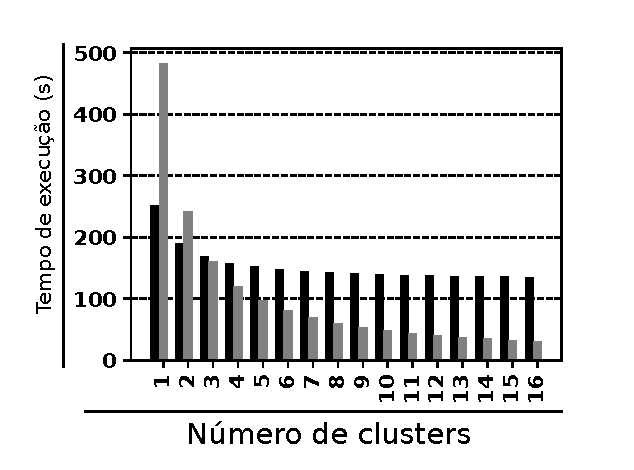
\includegraphics[width=7cm, keepaspectratio]{figs/fntime.pdf}
    \label{fig:fig7}
\end{figure}
\end{frame}

\begin{frame}\frametitle{Gasto energético da aplicação FN}
\begin{itemize}
\item Ganho mínimo de 23.2\% (5 \textit{clusters}) e máximo de 70.9\% (16 \textit{clusters})
\end{itemize}
\begin{figure}
    \centering
    
\includegraphics[width=4cm, keepaspectratio]{figs/legend.pdf}
    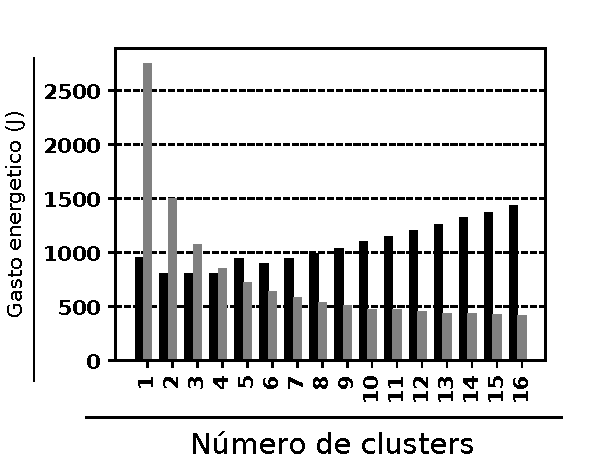
\includegraphics[width=7cm, keepaspectratio]{figs/fnpower.pdf}
    \label{fig:fig8}
\end{figure}
\end{frame}

\begin{frame}\frametitle{Tempos de execução da aplicação LU}
\begin{itemize}
\item Ganho médio de 60.5\% independente do número de \textit{clusters}
\end{itemize}
\begin{figure}
    \centering
    
\includegraphics[width=4cm, keepaspectratio]{figs/legend.pdf}
    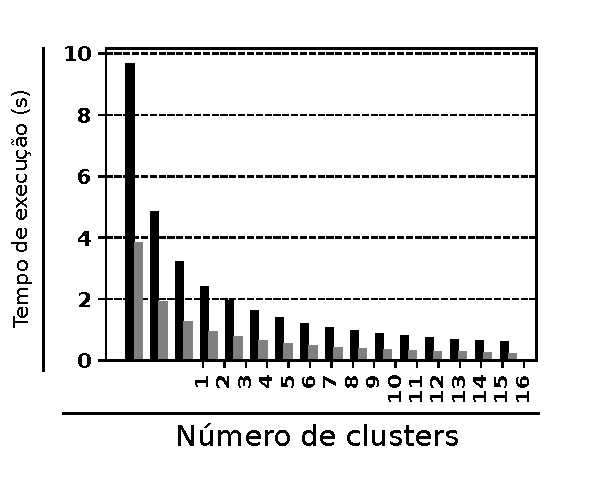
\includegraphics[width=7cm, keepaspectratio]{figs/lutime.pdf}
    \label{fig:fig9}
\end{figure}
\end{frame}

\begin{frame}\frametitle{Gasto energético da aplicação LU}
\begin{itemize}
\item Ganho mínimo de 87.6\% (1 \textit{clusters}) e máximo de 92.7\% (16 \textit{clusters})
\end{itemize}
\begin{figure}
    \centering
    
\includegraphics[width=4cm, keepaspectratio]{figs/legend.pdf}
    \label{fig:fig8}
    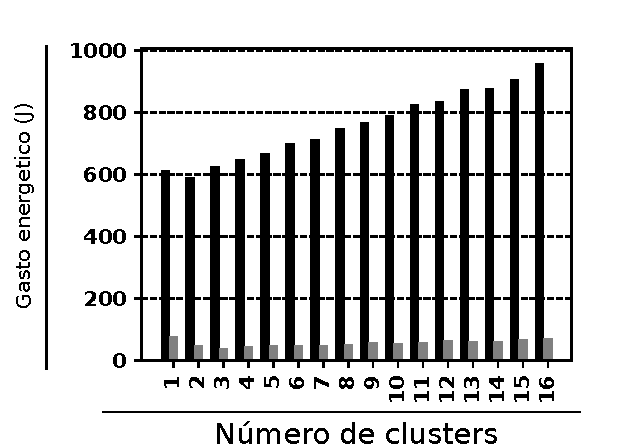
\includegraphics[width=7cm, keepaspectratio]{figs/lupower.pdf}
    \label{fig:fig8}
\end{figure}
\end{frame}

\section{Conclusões}
\begin{frame}\frametitle{Conclusões}
    \begin{itemize}
        \item Redução significativa no tempo de execução das aplicações
	    \begin{itemize}
        	\item FN com redução máxima de 77.6\%
    		\item LU com redução média de 60.5\%
    	\end{itemize}
        \item Redução significativa também no consumo energético.
	    \begin{itemize}
        	\item FN com redução máxima de 70.9\%
    		\item LU com redução máxima de 92.7\%
    	\end{itemize}
    	\item Grande potencial de otimização
    	\item Otimizar as demais aplicações do \textit{benchmark}
    \end{itemize}

\end{frame}

%Fim
\begingroup
    \makeatletter
    \setlength{\hoffset}{-.5\beamer@sidebarwidth}
    \makeatother
    \begin{frame}[plain,t,noframenumbering]
        \titlepage
    \end{frame}
\endgroup

% \section{Extra}
% \begin{frame}\frametitle{Extra}
% \begin{figure}[t]
%   \begin{minipage}[b]{0.9\textwidth}
% 	\centering
%     % \caption{\textit{tiling} 2D.}
%     \includegraphics[height=5cm]{figs/tile.pdf} \\
%     % Fonte:~\cite{rocha17}
% 	\label{fig:block2d}
%   \end{minipage}
% \end{figure}
% \end{frame}

\section{Referências}
\begin{frame}\frametitle{Referências}
    {\tiny
        \bibliographystyle{abbrv}
        \bibliography{bibliography}}
\end{frame}

\end{document}
